


\documentclass[a4paper,11pt]{article} % ce document est un article sur une feuille A4, police taille 11
\usepackage[utf8]{inputenc}
\usepackage[T1]{fontenc} % compatible avec les accents
\usepackage{biblatex} %Imports biblatex package
\addbibresource{GAN video games.bib} %Import the bibliography file

\usepackage[french]{babel} % rédigé en français

\usepackage{graphicx} % gestion des images
\usepackage{array} % gestion des tableaux
\usepackage{csquotes} % gestion des guillemets
\usepackage{fourier} % utilise une autre police que celle par défaut (Computer Modern)

\title{Les réseaux antagonistes génératifs dans les jeux vidéos}
\author{Sarah Pirard}
\date{Décembre 2022}

\begin{document}

\maketitle

\section{Introduction}
Qu'est-ce qu'un réseau antagoniste génératif? Un réseau antagoniste génératif, également communément appelé "GAN" (generative adversarial network) est une classe d'algorithme qui permet de créer des images de synthèse à partir d'échantillons. Le principe est de mettre en opposition deux réseaux, en premier lieu le générateur, qui génère une image au discriminateur sur base d'un échantillon qui doit détecter si l'image est réelle ou si elle résulte de la création du générateur (Alankrita et al., 2021). Ce processus a été mis en place en 2014 par (Goodfellow et al.).Il en existe de nombreuses variantes à ce jour (Asimopoulos et al., 2022). Les GAN sont actuellement utilisés dans de nombreux domaines notamment dans l'imagerie médicale et le traitement d'image et de vidéo. Le domaine qui nous intéresse dans cet article est le domaine des jeux vidéos. 

\begin{figure}[h] % insère une figure ici (h = "here")
  \centering % centre la figure
  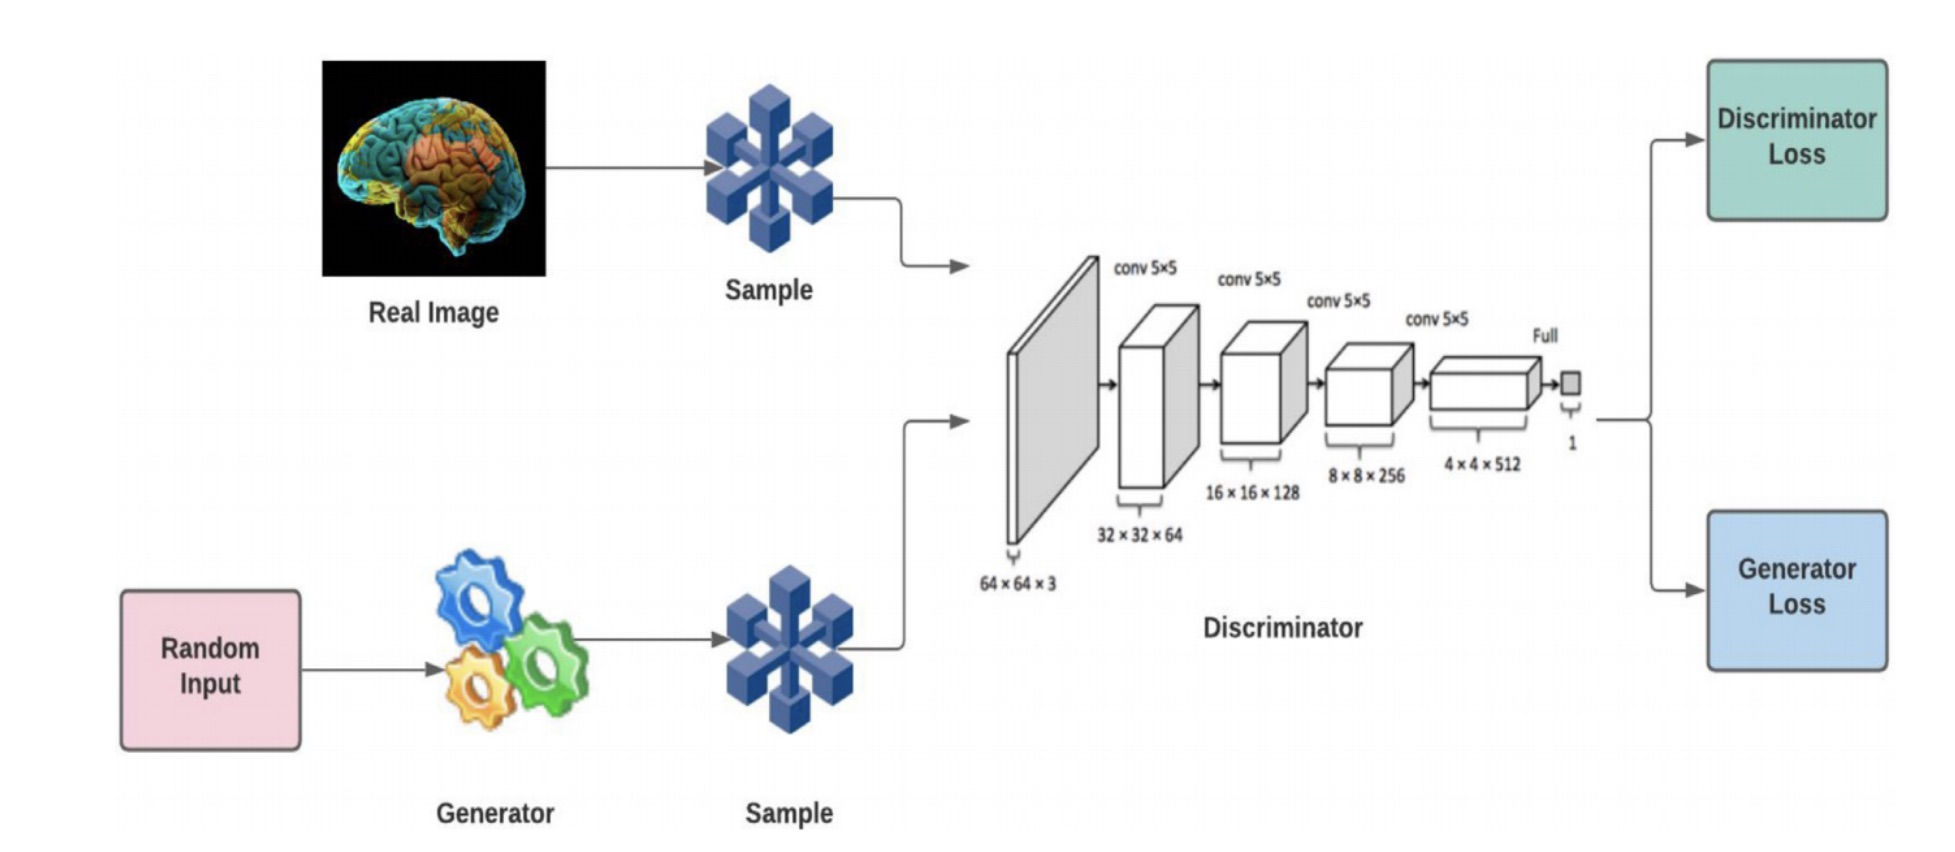
\includegraphics[scale=0.17]{GAN}


  \caption{fonctionnement d'un réseau antagoniste génératif} % nom de l'image
\end{figure}

\section{Quelles applications dans les jeux vidéos?}

Les generative adversarial networks se sont montrés particulièrement efficaces en matière de PCG (Procedural Content Generation) dans le déploiement de nouveaux niveaux de jeux. Le PCG peut être utilisé pour générer des niveaux de jeu, des règles ou encore des textures pour les éléments graphiques. Il permet notamment de créer des mondes de jeux complexes en évitant de produire une surcharge de travail conséquente aux designers graphiques (Hendrikx et al, 2011).











\end{document}
